%% Lab Report for EEET2493_labreport_template.tex
%% V1.0
%% 2019/01/16
%% This is the template for a Lab report following an IEEE paper. Modified by Francisco Tovar after Michael Sheel original document.


%% This is a skeleton file demonstrating the use of IEEEtran.cls
%% (requires IEEEtran.cls version 1.8b or later) with an IEEE
%% journal paper.
%%
%% Support sites:
%% http://www.michaelshell.org/tex/ieeetran/
%% http://www.ctan.org/pkg/ieeetran
%% and
%% http://www.ieee.org/

%%*************************************************************************
%% Legal Notice:
%% This code is offered as-is without any warranty either expressed or
%% implied; without even the implied warranty of MERCHANTABILITY or
%% FITNESS FOR A PARTICULAR PURPOSE! 
%% User assumes all risk.
%% In no event shall the IEEE or any contributor to this code be liable for
%% any damages or losses, including, but not limited to, incidental,
%% consequential, or any other damages, resulting from the use or misuse
%% of any information contained here.
%%
%% All comments are the opinions of their respective authors and are not
%% necessarily endorsed by the IEEE.
%%
%% This work is distributed under the LaTeX Project Public License (LPPL)
%% ( http://www.latex-project.org/ ) version 1.3, and may be freely used,
%% distributed and modified. A copy of the LPPL, version 1.3, is included
%% in the base LaTeX documentation of all distributions of LaTeX released
%% 2003/12/01 or later.
%% Retain all contribution notices and credits.
%% ** Modified files should be clearly indicated as such, including  **
%% ** renaming them and changing author support contact information. **
%%*************************************************************************

\documentclass[journal]{IEEEtran}

% *** CITATION PACKAGES ***
\usepackage[style=ieee]{biblatex} 
\bibliography{example_bib.bib}    %your file created using JabRef

% *** MATH PACKAGES ***
\usepackage{amsmath}
\usepackage{amsfonts}
\usepackage{comment}
\usepackage{amssymb} % Este paquete contiene el símbolo \approxeq

\usepackage{tabularx} % en el preámbulo
\usepackage{caption}
\captionsetup{font=small, labelfont=bf, textfont=normalfont}


% *** PDF, URL AND HYPERLINK PACKAGES ***
\usepackage{url}
% correct bad hyphenation here
\hyphenation{op-tical net-works semi-conduc-tor}
\usepackage{graphicx}  %needed to include png, eps figures
\usepackage{subcaption}
\usepackage{float}  % used to fix location of images i.e.\begin{figure}[H]

\begin{document}

% paper title
\title{Polarización del Transistor BJT\\ \small{Práctica No. 4}}

% author names and affiliations
\author{
    \IEEEauthorblockN{Flores Cornejo Gustavo Mauricio, Muñoz Reyes Arturo Yabed, Morales Vásquez Miguel Ehecatl}\\
    \IEEEauthorblockA{\textit{Unidad Profesional Interdisciplinaria en Ingeniería y Tecnologías Avanzadas, IPN}}
}
        
% The report headers
\markboth{1MV12 Fundamentos de Electrónica. Práctica 4, Abril 2026}%do not delete next lines
{Shell \MakeLowercase{\textit{et al.}}: Bare Demo of IEEEtran.cls for IEEE Journals}

% make the title area
\maketitle

% As a general rule, do not put math, special symbols or citations
% in the abstract or keywords.
\begin{abstract}
    This paper analyzes the behavior and operation of the Bipolar Junction Transistor (BJT) under a fixed bias configuration. 
    Using NPN 2N2222 transistors, the terminals were identified, and the operating regions—cutoff, saturation, and active—were experimentally determined. 
    The flow of collector ($I_C$) and base ($I_B$) currents was examined, alongside the variation of the $\beta$ parameter under different voltage and resistance levels. 
    The results, obtained through direct measurements and simulations, allowed for a comparison between real values and manufacturer specifications, confirming the 
    BJT's utility as a switch and linear amplifier in DC electronic circuits.
\end{abstract}

\section{Introducción}
    % Here we have the typical use of a "W" for an initial drop letter
    % and "RITE" in caps to complete the first word.
    % You must have at least 2 lines in the paragraph with the drop letter
    % (should never be an issue)

    \IEEEPARstart{D}urante el periodo de 1904 a 1947, el tubo de vacío fue el componente electrónico de mayor interés y 
    desarrollo, debido a su capacidad de amplificar señales analógicas, impulsado significativamente por la industria de la radio y televisión
    en sus años posteriores. Sin embargo en 1947, la aparición del transistor  marcaría un cambio importante en la industria
    de la electrónica.  Este nuevo dispositivo de estado sólido de tres terminales ofrecía grandes ventajas frente a su antecesor:
    dimensiones más pequeñas, menor peso, baja disipación de calor y fundamentalmente,  una mayor eficiencia energética al consumir
    una fracción de la potencia requerida por las válvulas de vacío.
 
    Gracias a estas propiedades y a su versatilidad para operar como interruptor electrónico, el transistor se integró rápidamente en 
    a arquitectura de los sistemas informáticos. La evolución en las técnicas de diseño y fabricación ha permitido reducir su escala de 
    centímetros a nanómetros, facilitando la construcción de microprocesadores de alta densidad. Este avance ha sido el pilar tecnológico 
    que dio paso a la computación móvil, los sistemas embebidos y los dispositivos de control que definen la tecnología contemporánea.

\section{Objetivos}
    \subsection{Objetivo General}
    Explicar el funcionamiento del transistor BJT con una configuración de polarización fija y  diseñar circuitos que provean algún comportamiento deseado.

    \subsection{Objetivos Particulares}
    \begin{enumerate}
        \item Identificar el colector, base y emisor del transistor.
        \item Comprender el flujo de las corrientes de colector y base.
        \item Analizar y comprender el comportamiento de la beta ante variaciones de voltaje. 
        \item Comprender el funcionamiento de las zonas de corte-saturación.
    \end{enumerate}

\section{Marco teórico}
    \subsection{El transitor BJT}
        Un transistor de unión bipolar (BJT, por sus siglas en inglés) es un dispositivo semiconductor 
        constituido por tres capas de material dopado, las cuales forman dos uniones P-N y, por consiguiente, 
        dos regiones de agotamiento o empobrecimiento. Dependiendo de la configuración de estas capas, 
        el dispositivo se clasifica en tipo NPN (dos capas de material tipo $n$ y una central tipo $p$) 
        o tipo PNP (dos capas tipo $p$ y una central tipo $n$), tal como se ilustra en la Figura 1. 
        Sus terminales se identifican como Emisor (E), Base (B) y Colector (C).
        
        \begin{figure}[H] % SIN asterisco y con H mayúscula
        \centering
            % --- Subfigura (a) NPN ---
            \begin{subfigure}[b]{0.47\columnwidth} % 45% de la COLUMNA
                \centering
                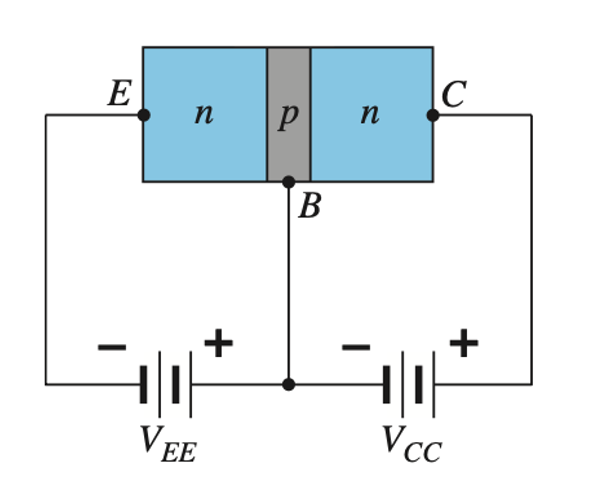
\includegraphics[width=\textwidth]{IMAGENES/Transistor_NPN.png}
                \caption{Transistor npn.}
                \label{fig:npn}
            \end{subfigure}
            \hfill % Esto las separa un poco dentro de la columna
            % --- Subfigura (b) PNP ---
            \begin{subfigure}[b]{0.45\columnwidth} % 45% de la COLUMNA
                \centering
                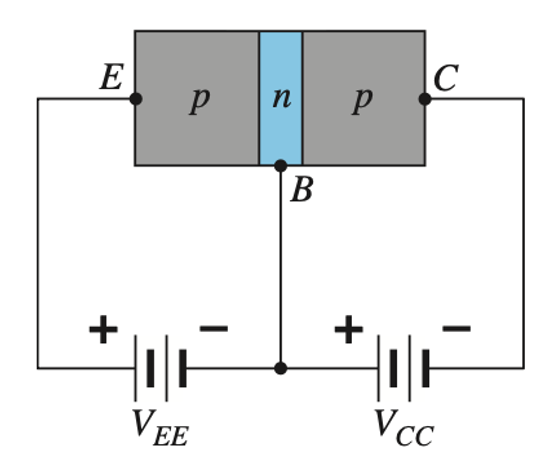
\includegraphics[width=\textwidth]{IMAGENES/Transistor_PNP.png}
                \caption{Transistor pnp.}
                \label{fig:pnp}
            \end{subfigure}
    
            % --- Pie de foto principal ---
            \caption{Configuraciones básicas del transistor de unión bipolar.}
            \label{fig:bjt_types}
        \end{figure}
   
        Constructivamente, el emisor presenta un nivel de dopaje elevado para maximizar la inyección de portadores,
        la base cuenta con un dopaje ligero y un espesor reducido, mientras que el colector posee un dopaje intermedio. 
        El término 'bipolar' hace referencia a que el mecanismo de conducción y la inyección de carga dependen del flujo tanto de electrones como de huecos.

    \subsection{Portadores de carga}
        El funcionamiento del BJT se basa en la interacción de los portadores de carga, los cuales se definen como las partículas elementales encargadas del 
        transporte de corriente eléctrica en el semiconductor. En un material tipo $n$ (negative) el electrón se denomina portador mayoritario debido a su abundancia, 
        mientras que el hueco actúa como portador minoritario. Por el contrario, en un material tipo $p$ (positive) el hueco es el portador mayoritario y el electrón el minoritario. 
    
    \subsection{Region de empobrecimiento}
        La unión de estos materiales da origen a la región de empobrecimiento, una zona carente de portadores libres que se forma debido a la 
        recombinación de electrones y huecos en la interfaz. Este proceso deja tras de sí iones dopantes fijos (positivos en el lado $n$ y negativos en el lado $p$),
        lo que establece un campo eléctrico interno . Este campo genera una barrera de potencial que impide el flujo portadores mayoritarios.
    
    \subsection{Funcionamiento}
        Tomando como ejemplo un transistor pnp y analizando el flujo de huecos (iones positivos), al polarizar la unión base-emisor
        como se muestra en la Figura 2 se obtiene el mismo comportamiento al de un diodo polarizado en directa. En este estado, el ancho de la 
        región de empobrecimiento se reduce permitiendo un flujo de huecos (portador mayoritario) del material p al n. Por otro lado, 
        en la Figura 3 se muestra qué sucede si se polariza la unión base-emisor, la situación presentada es semejante a la de un diodo 
        polarizado en inversa. La región de empobrecimiento se agranda impidiendo el paso de portadores mayoritarios, resultando únicamente en un flujo de portadores minoritarios.
    
        \begin{figure}[H]%[!ht]
            \centering
            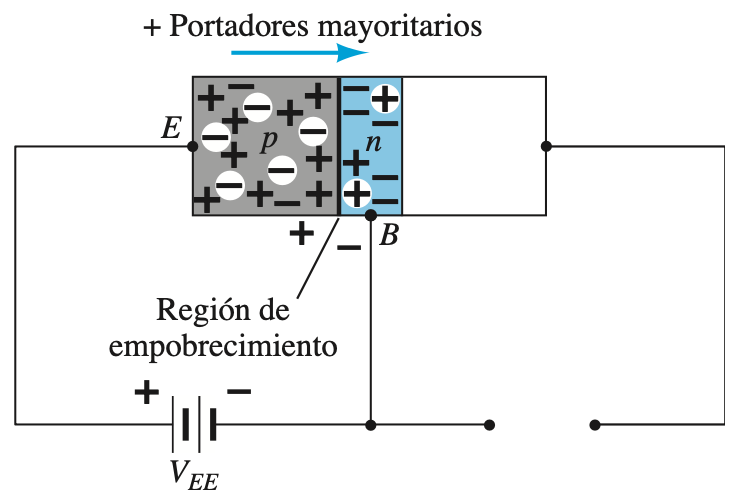
\includegraphics[width=0.35\textwidth]{IMAGENES/Polarizacion_directa.png}
            \caption{Unión polarizada en directa.
}
            \label{fig:pnp_direct}
        \end{figure}

        \begin{figure}[H]%[!ht]
            \centering
            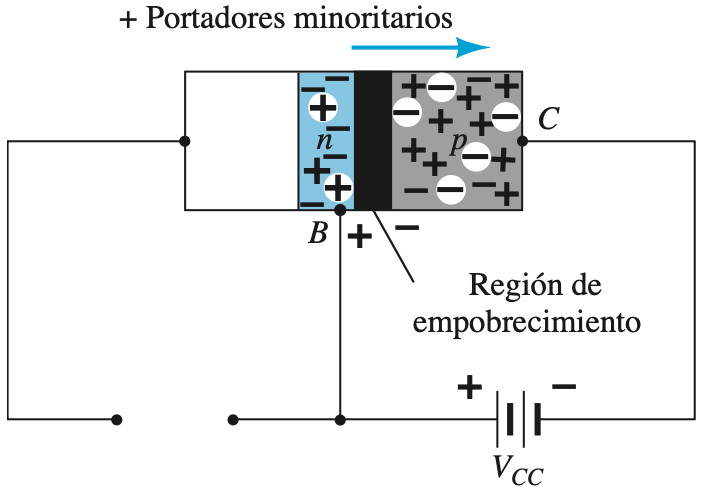
\includegraphics[width=0.33\textwidth]{IMAGENES/Polarizacion_inversa.png}
            \caption{Unión polarizada en inversa.}
            \label{fig:pnp_inverse}
        \end{figure}

        Si se aplican ambos potenciales de polarización al transistor pnp y analizamos qué sucede notamos que el emisor al 
        ser de un material tipo $p$, está saturado de huecos, los cuales son repelidos por el positivo de la fuente $V_{EE}$ provocando 
        que pasen directamente al material tipo $n$. Recordando que el material tipo $n$ está poco dopado, no tiene tantos electrones 
        para combinarse con los huevos por lo que solo una pequeña parte de estos podrá regresar al negativo de la fuente $V_{EE}$, 
        como se indica en la Figura 4. Esos huecos sobrantes en la base pasan a convertirse en portadores minoritarios del material tipo $n$, 
        esto es importante ya que como se mencionó anteriormente, un diodo en inversa sólo permite el flujo de portadores minoritarios.

        \begin{figure}[H]%[!ht]
            \centering
            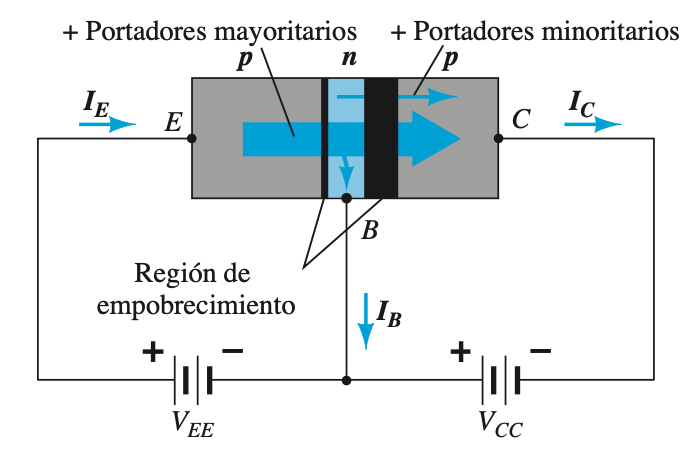
\includegraphics[width=0.35\textwidth]{IMAGENES/FlujoPortadores_pnp.png}
            \caption{Flujo de portadores mayoritarios y minoritarios de un transistor pnp.}
            \label{fig:flujoPortadores}
        \end{figure}

        Los huecos ahora convertidos en portadores minoritarios pasan con facilidad a través de la región de empobrecimiento hacia el colector, 
        debido a que son empujados por el campo eléctrico formado en esta región por la polarización en inversa,  y a su vez, son atraídos por la 
        terminal negativa de la fuente $V_{CC}$ , al llegar al colector estos mueren al combinarse con los electrones provenientes de la fuente. 
        
        Aplicando la ley de corrientes de Kirchhoff al transistor de la Figura 4.
        \begin{equation}
            I_E = I_C + I_B
            \label{ec:correintesTransistor}
        \end{equation}

    \subsection{Corrente de Fuga}
        La corriente en el colector no solo está compuesta por el flujo de huecos (portadores mayoritarios en el material p del colector),  
        sino también de un flujo de portadores minoritarios llamada corriente de fuga y se le da el símbolo de $I_{CO}$. Esta corriente es 
        análoga a la corriente de saturación de un diodo Is  y por lo tanto es sensible a la temperatura, 
        dependiendo del caso puede afectar seriamente al uso del transistor, sin embargo generalmente puede ignorarse  ($I_{CO} \approx 0 $).
        
        La corriente total que pasa por el colector está determinada por:
        \begin{equation*}
            I_{C} = I_{C_{\text{mayoritarios}}} + I_{CO_{\text{minoritarios}}}
            \label{eq:corriente_colector}
        \end{equation*}
    
    \subsection{Configuración Emisor Común}
        Existen tres configuraciones fundamentales para la operación de un transistor de unión bipolar (BJT): base común, colector común y 
        emisor común. Para describir el comportamiento eléctrico de cada una, es necesario analizar dos conjuntos de curvas características:
        las de entrada (parámetros de control) y las de salida (parámetros de carga).
    
        La configuración de Emisor Común es la más utilizada en la por su alta ganancia tanto en voltaje como en corriente, 
        lo que le otorga una gran versatilidad para el diseño de amplificadores y circuitos de conmutación de potencia. Recibe su 
        nombre debido a que la terminal del emisor sirve como punto de referencia común tanto para el circuito de entrada (Base) 
        como para el de salida (Colector), vease en la Figura 5.

        \begin{figure}[H]%[!ht]
        \centering
            % --- Subfigura (a) NPN ---
            \begin{subfigure}[b]{0.47\columnwidth} % 45% de la COLUMNA
                \centering
                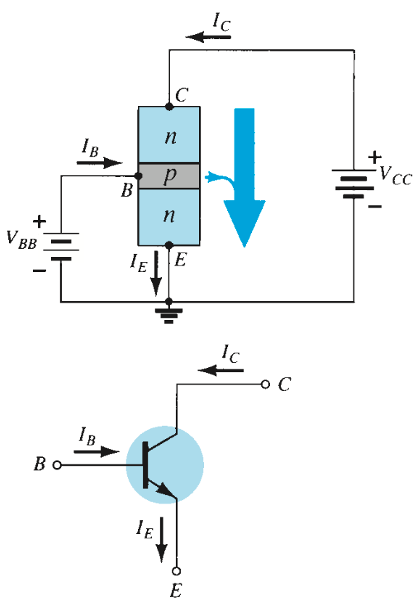
\includegraphics[width=\textwidth]{IMAGENES/EmisorComun_npn.png}
                \caption{Transistor npn.}
                \label{fig:Emisor_com_npn}
            \end{subfigure}
            \hfill % Esto las separa un poco dentro de la columna
            % --- Subfigura (b) PNP ---
            \begin{subfigure}[b]{0.47\columnwidth} % 45% de la COLUMNA
                \centering
                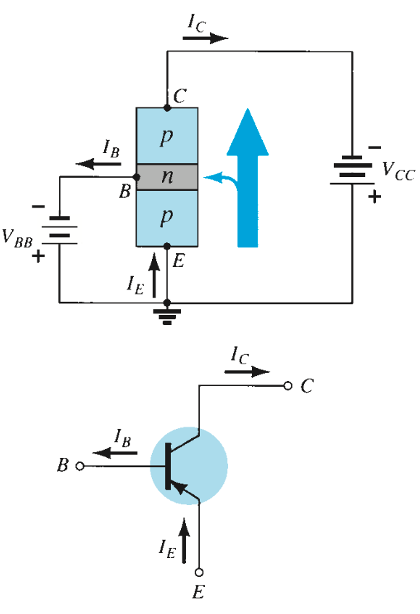
\includegraphics[width=\textwidth]{IMAGENES/EmisorComun_pnp.png}
                \caption{Transistor pnp.}
                \label{fig:Emisor_com_pnp}
            \end{subfigure}
            % --- Pie de foto principal ---
            \caption{Configuraciones básicas del transistor de unión bipolar.}
            \label{fig:emisorComun_types}
        \end{figure}
        El comportamiento del dispositivo se rige por la interacción entre sus mallas;  el circuito de entrada que 
        relaciona la corriente de base ($I_B$) con el voltaje base-emisor ($V_{BE}$). Asi como el circuito de 
        salida que relaciona la corriente de colector ($I_C$) con el voltaje colector-emisor ($V_{CE}$).

    \subsection{El Parámetro Beta ($\beta$) como factor de amplificación}
        En la configuración de emisor común, la relación entre la corriente de salida ($I_C$) y la corriente de entrada ($I_B$), 
        denominada como beta ($\beta$), define la ganancia de corriente de CD. Este parámetro es fundamental, ya que representa el 
        factor de amplificación del dispositivo; un pequeño incremento en la corriente de base produce un aumento significativamente 
        mayor en el colector, permitiendo el control del flujo de potencia.

        En general para cualquier configuración:
        \begin{equation}
            \beta = \frac{I_C}{I_B} 
        \end{equation}

        Desbejando el valor de $I_C$ se obtiene la relacion de amplificación antes mencionada: 
        \begin{equation}
            I_C= \beta I_B
        \end{equation}

        Sustituyendo en la ecuación \eqref{ec:correintesTransistor}:
        \begin{equation}
            I_E= (\beta + 1)I_B
        \end{equation}

        Obteniendo una relacion entre la coriente de entrada y la corriente del emisor ($I_E$). 
        Dado que en la mayoría de transistores usualmente es un valor mucho mayor que 1 ($\beta \gg 1$), 
        entonces podemos inferir una relación entre la corriente de colecor y la corriente del emisor.
        \begin{equation*}
            \beta + 1 \gg \beta
        \end{equation*}
        De forma muy aproximada:
        \begin{equation*}
            I_E \approx (\beta)I_B
        \end{equation*}
        Por lo tanto:
        \begin{equation}
            I_C \approxeq I_B
        \end{equation}

    \subsection{Curvas características del BJT en emisor común}
        La curva característica de entrada representa la relación entre los parametros de entrada
         ($V_{BE}$ e $I_B$), para distintos valores de voltaje colector-emisor ($V_{CE}$).
        Como se ve en la Figura \ref{fig:carac_base} esta presenta un comportamiento exponencial similar al de un diodo polarizado en directa,
        en el cual $I_B$ es prácticamente nula hasta que la tensión alcanza el voltaje de umbral o barrera.

        \begin{figure}[H]%[!ht]
            \centering
            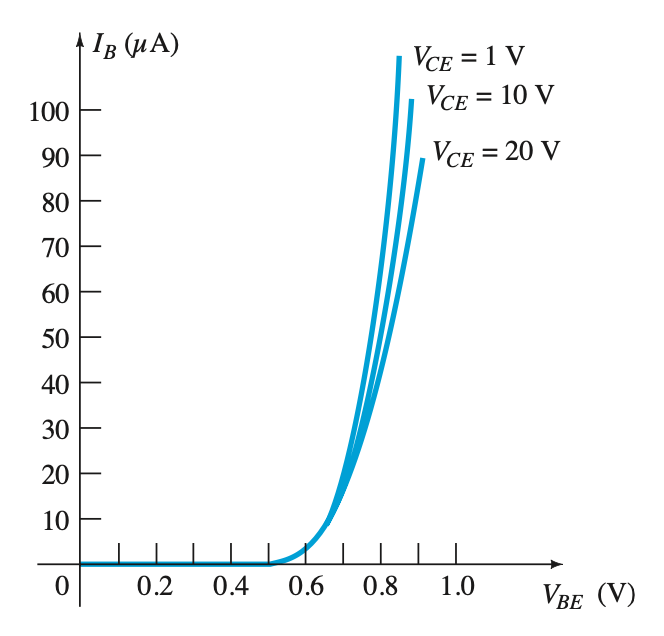
\includegraphics[width=0.34\textwidth]{IMAGENES/Caracteristicas_base.png}
            \caption{Características de entrada para un transistor de silicio en emisor común.}
            \label{fig:carac_base}
        \end{figure}

        Es decir, una vez que un transitor se "enciende", se puede suponer que el voltaje base-emisor sera:
        \begin{equation}
            V_{BE} = 0.7 V
            \label{ec:Voltaje_BE}
        \end{equation} 

        Al observar la Figura \ref{fig:carac_salida}, se aprecia que $I_B$ se mide en $\mu$A mientras que $I_C$ en mA,
        reflejando la amplificación del BJT. La pendiente positiva en las curvas de salida se debe que
        al aumentar el voltaje en inversa $V_{CB}$, la región de empobrecimiento se expande hacia la base,
        reduciendo su ancho efectivo. Esta disminución en el ancho de la base reduce la recombinación de portadores,
        facilitando su paso al colector e incrementando ligeramente $I_C$ conforme aumenta $V_{CE}$

        \begin{figure}[H]%[!ht]
            \centering
            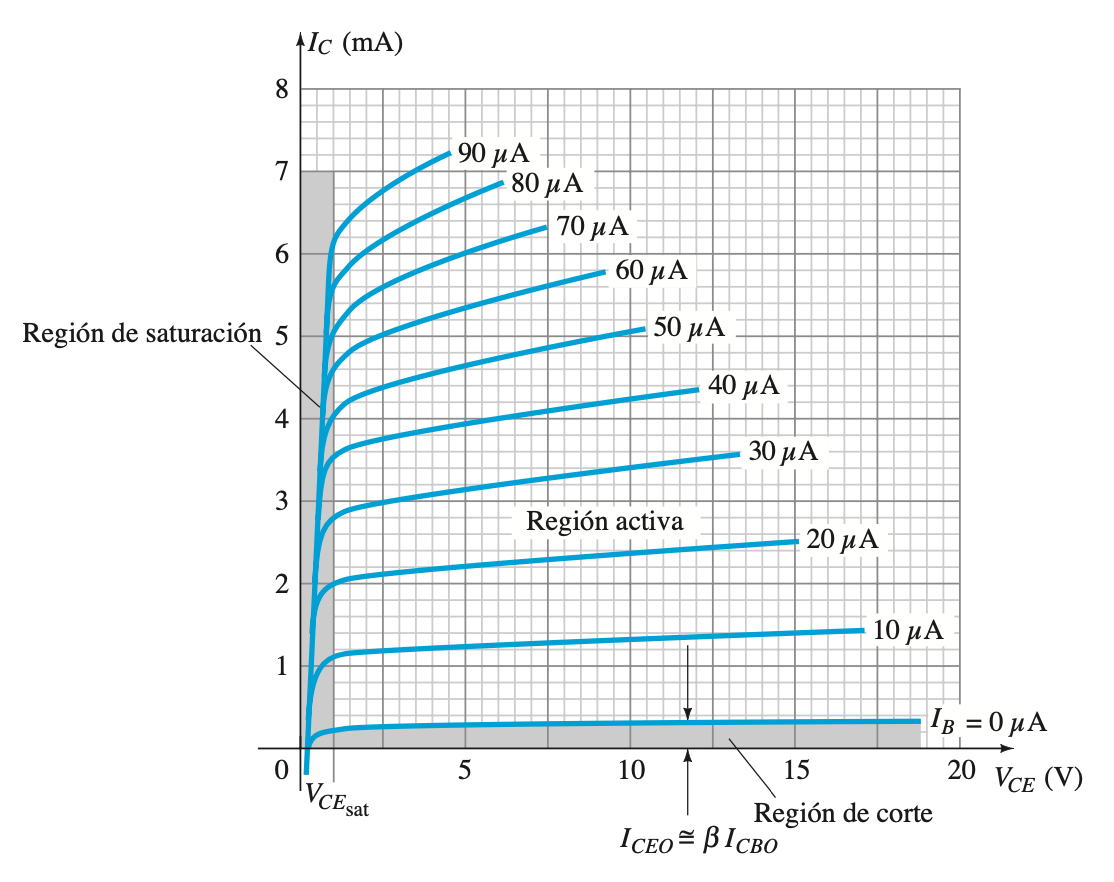
\includegraphics[width=0.45\textwidth]{IMAGENES/Caracteristicas_salida.png}
            \caption{Características de salida para un transistor de silicio en emisor común.}
            \label{fig:carac_salida}
        \end{figure}
    
    \subsection{Regiones de operación}
        Para comprender visualmente cómo opera el transistor en cada una de las distintas regiones de la 
        Figura \ref{fig:carac_salida}, es útil compararlo con el funcionamiento de un grifo de agua:

        \begin{figure} [H]%[!ht]
            \centering
            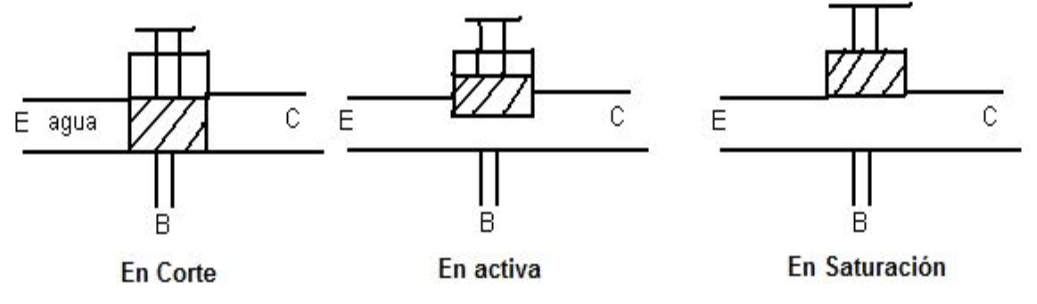
\includegraphics[width=0.45\textwidth]{IMAGENES/Estados_transistor.png}
            \caption{Ejemplo gráfico de las tres regiones de operación.}
            \label{fig:estados_transitor}
        \end{figure}

        \subsubsection{Región de Corte (Grifo cerrado)}
            En este estado, no hay una corriente aplicada en la base ($I_B = 0$). Al no haber "presion" que active el transistor,
            el transistor impide el paso de la corriemte entre el colector y el emisor. Sin embargo, esta presente 
            una pequeña llama corriente $I_{CEO}$ ocacionada por la corriente de fuga de la union en inversa ($I_{CO}$).

        \subsubsection{Región Activa (Flujo controlado)}
            Es la zona de amplificación lineal. Aquí, la apertura del grifo es proporcional a la fuerza aplicada en la perilla; es decir,
            $I_C$ varía de forma lineal y proporcional a los cambios en $I_B$. La señal de salida sigue fielmente las variaciones 
            de la entrada, pero a una escala mucho mayor.

        \subsubsection{Región de Saturación (Grifo Abierto al Máximo)}
            En este punto, por más que se incremente la corriente de base, el flujo en el colector ha alcanzado su límite máximo permitido
            por la fuente de alimentación ($V_{CC}$) y las resistencias del circuito.

    \subsection{Punto de operación Q}
        El punto de operación, también llamado punto quiesciente (inmóvil o inactivo) representa un punto de la gráfica de características de salida (Fig \ref{fig:carac_salida}), 
        este viene determinado por valores especificos de corriente de colector y voltaje de colector-emisor. Dependiendo de como queramos que funcione el transitor el punto Q se
        hubicara en distintas zonas de la gráfica.
            
    \subsection{El transistor como aplificador}
        Para emplear el transistor en aplicaciones de amplificación, es necesario que el punto de operación (punto Q) se ubique aproximadamente en la zona media de la región activa.
        Esta selección estratégica maximiza la excursión de la señal de salida, evitando recortes por saturación o corte que comprometan la fidelidad de la señal amplificada.

    \subsection{Polarización Fija}
        El término polarización se refiere a la aplicación de voltajes de corriente directa (CD) con el objetivo de establecer 
        niveles fijos de corriente y voltaje que definan el estado operativo del dispositivo. Dentro de las distintas maneras de polarizar
        un transitor, la mas elemental de ellas es la polarización fija, la cual se ejemplifica en la Figura \ref{fig:polarizacion_fija}.
        \begin{figure} [H]
            \centering
            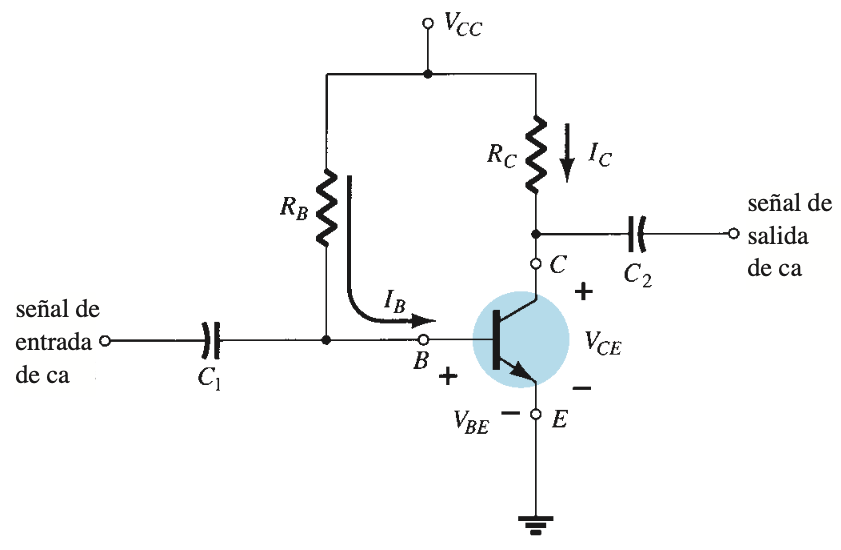
\includegraphics[width=0.4\textwidth]{IMAGENES/Polarizacion_fija.png}
            \caption{Polarización Fija.}
            \label{fig:polarizacion_fija}
        \end{figure}
    
    \subsection{Recta de Carga de CD}
        La ubicación del punto Q se analiza mediante la recta de carga, una representación gráfica de la ecuación de malla del colector que interseca las curvas 
        características del dispositivo. Esta recta delimita todos los posibles estados de funcionamiento ($I_C, V_{CE}$) que el 
        transistor puede adoptar para una red de polarización y carga específicas.
        \begin{figure} [H]
            \centering
            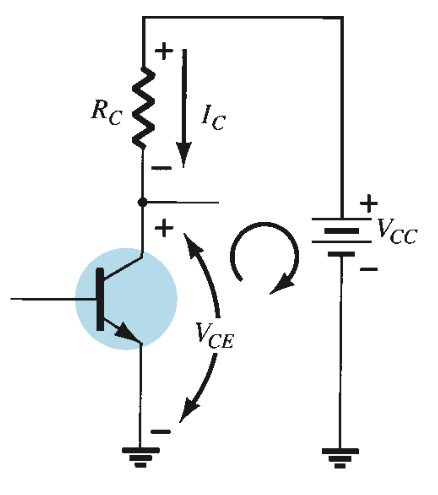
\includegraphics[width=0.2\textwidth]{IMAGENES/Malla_colectorEmisor.png}
            \caption{Malla colector-emisor.}
            \label{fig:Malla_colectorEmisor}
        \end{figure}

        Si aplicamos la ley de voltajes de kirchoff a la malla de la Figura \ref{fig:Malla_colectorEmisor},
        se obtiene la ecuación de la recta de carga
        \begin{equation*}
            V_{CE} + I_C R_C - V_{CC} = 0
        \end{equation*}
        \begin{equation}
            V_{CE} =  V_{CC} + I_C R_C
        \end{equation}
        \begin{figure}[H]
            \centering
            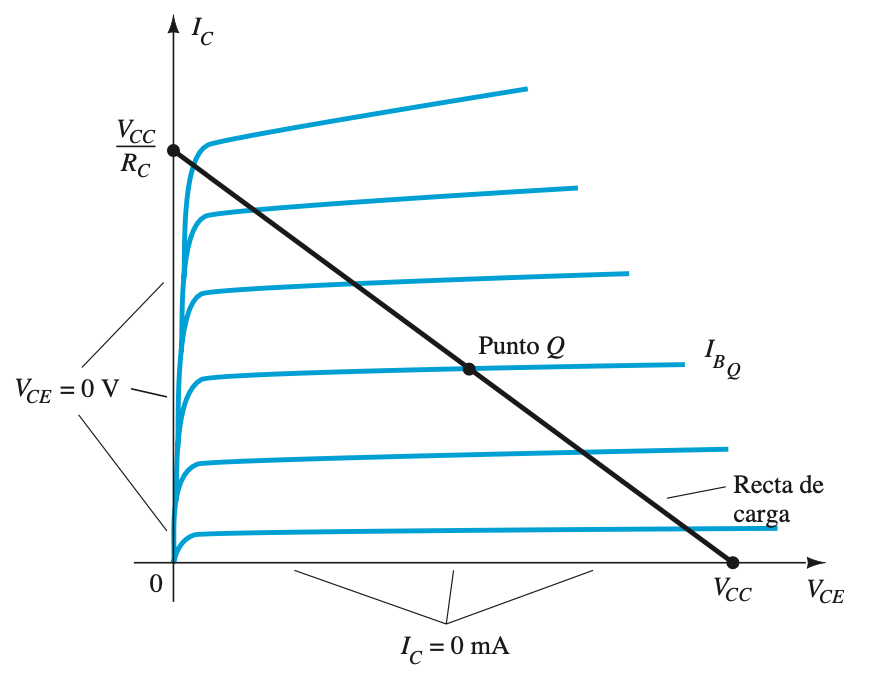
\includegraphics[width=0.45\textwidth]{IMAGENES/Recta_carga.png}
            \caption{Recta de carga para la configuración de polarización fija.}
            \label{fig:recta_carga}
        \end{figure}

    \subsection{Redes de Conmutación}
        Cuando el objetivo no es la amplificación lineal, sino el control de cargas, el transistor se configura para 
        operar exclusivamente en sus estados críticos. En este esquema, la base es excitada por una señal de control (como la salida de un microcontrolador),
        lo que obliga al dispositivo a alternar entre las regiones de corte y saturación. En este modo de operación, conocido como conmutación (switch), 
        el BJT actúa como un interruptor electrónico: en corte, el circuito permanece abierto e impide el paso de corriente; en saturación, el transistor 
        permite el flujo máximo hacia la carga con una caída de tensión mínima ($V_{CE_{sat}}$).
        \begin{figure} [H]
            \centering
            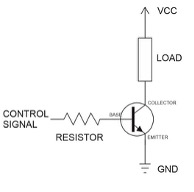
\includegraphics[width=0.2\textwidth]{IMAGENES/Switching_transitor.jpg}
            \caption{Configuración de un transitor para conmutación.}
            \label{fig:switching_transitor.jpg}
        \end{figure}

    \subsection{Potencia Máxima}
    La operación del transistor está restringida por la curva de potencia máxima disipada ($P_{max}$),
    la cual representa el límite térmico que el dispositivo puede soportar sin sufrir daños permanentes.
    Dada por la ecuación:
    \begin{equation*}
        P_{max} = V_{CE} I_C 
    \end{equation*}

    Para garantizar la integridad del componente, el punto de operación (punto Q) y la recta de carga 
    deben situarse siempre por debajo de esta curva dada por el fabricante.

    \subsection{Valores Nominales y Parámetro $h_{FE}$}
    Para el diseño y análisis de circuitos con el BJT, es necesario consultar los valores nominales especificados por el fabricante.
    Estos valores representan los límites que no deben excederse para evitar dañar del dispositivo. Para la configuración
    emisor comun serian: $V_{CE_{max}} = V_{CEO}$, $I_{C_{max}}$ y $P_D = P_{max}$
    
    Por otro lado, la ganancia de corriente de $\beta$ se identifica en las hojas de datos como el parámetro $h_{FE}$ 
    (parámetro híbrido de emisión común). Es importante notar que $h_{FE}$ no es un valor estático. Depende de la temperatura,
    la corriente $I_C$ y las las tolerancias del fabricante.

    \subsection{Relaciones importantes}
    Recapitulando, para el análizis de cualquier configuración en CD sera necesario
    tener presente las siguiente ralaciones básicas de un transistor:
    \begin{equation}
        V_{BE} = 0.7 V
    \end{equation}
    \begin{equation}
        I_E = (\beta + 1) I_B \cong I_C
    \end{equation}
    \begin{equation}
        I_C = \beta I_B
    \end{equation}

    
\section{Materiales}
Para el circuito mostrado en la "Figura~\ref{fig:circuito_base1}”, emplearemos:
\begin{itemize}
    \item 4 Diodos 1N4002
    \item 4 Resistencias de 330 $\Omega$
    \item 1 Resistencia de 1 $\Omega$
    \item 1 Transformador reductor con derivación central a 12 Vrms
    \item 1 Protoboard
    \item Cable para protoboard
\end{itemize}

En la "Figura~\ref{fig:circuito_base1}", podemos observar que se utilizan diodos 1N4001, por cuestiones de practicidad y de seguridad se emplearán diodos 1N4002 que soportan hata un voltaje inverso de 100V y una
corriente de hasta 1A. Cabe aclarar, que el circuito mostrado se propone como un rectificador de media onda, sin embargo, al conectar la derivación central del transformador y colocar los diodos como se muestra obtenemos 
en realidad un rectificador de onda completa.

\section{Análisis y Resultados}
\subsection{Comprtamiento del transformador}
En esta sección se presentan y analizan las mediciones fundamentales del transformador reductor. Iniciamos con la 
identificación de los devanados (primario y secundario) y su derivación central a partir de la medición de sus resistencias. 
Posteriormente, con el equipo energizado, se documentan los voltajes RMS para determinar su relación de transformación. 
Finalmente, se verifica el desfasamiento de 180 grados entre las terminales, comprobando la suma de potenciales de extremo a extremo.

Para la caracterización inicial sin energizar, se midió la resistencia de las terminales para identificar los devanados. 
El devanado primario registró una resistencia de 112.4 $\Omega $. Por su parte, el devanado secundario presentó una resistencia total 
de 1.8 $\Omega $ medido de extremo a extremo. Al medir desde los extremos hacia la derivación central, se obtuvo una lectura de 0.9 $\Omega $, 
lo cual representa exactamente la mitad de la medición total y confirma la simetría del componente.

Posteriormente, al conectar el transformador a la toma de corriente de 120 $Vrms$ , se registró un voltaje de salida en el primario de $V_p = 120 Vrms$ (igual al de la fuente)
y en el secundario presentó un voltaje de $V_s = 13.21 Vrms$ de extremo a extremo. Con los datos obtenidos, podemos determinar el valor de la relacion de transformación (n)
del componente, para esto se calculó la proporción entre el voltaje suministrado al devanado primario ($Vp$) y el voltaje medido en el devanado secundario ($V_s$). Obtenemos:

\[
        n = \frac{V_p}{V_s} = \frac{120}{13.21} = {9.08}
\]

Con esto podemos observar la relación de reducción, es decir, el cálculo arroja una relación de transformación de aproximadamente 9:1. Lo cual indica físicamente que por cada 9 espiras 
en el devanado primario, existe 1 espira en el secundario, confirmando la naturaleza reductora del transformador utilizado.

Al utilizar la derivación central del secundario como punto de referencia común (tierra) para el osciloscopio, se midieron simultáneamente los voltajes de las dos terminales restantes. 
Se pudo comprobar gráficamente un desfasamiento exacto de 180 grados  entre ambas señales como se muestra en la "Figura~\ref{fig:desfasamiento}".

\begin{comment}
\begin{figure}[H]%[!ht]
\begin {center}

\includegraphics[width=0.45\textwidth]{IMAGENES/TRANSFORMADOR.png}
\caption{Desfasamiento de 180 grados en el transformador.}
\label{fig:desfasamiento}
\end {center}
\end{figure}
\end{comment}

Este desfasamiento ocurre debido a la polaridad relativa inducida en la bobina. Según la Ley de Faraday, el flujo magnético alterno induce una diferencia de potencial a lo largo de 
todo el devanado secundario. Al "anclar" el centro físico de la bobina a 0V, el voltaje total se divide en dos mitades. En el instante en que la terminal superior es empujada hacia un 
potencial positivo máximo, la terminal inferior es forzada hacia un potencial negativo máximo de la misma magnitud para mantener la diferencia de potencial total. El resultado son dos 
señales senoidales que son el "espejo" la una de la otra.

Para corroborar la relación entre las señales, se procedió a medir con el osciloscopio la señal de extremo a extremo del secundario, omitiendo la derivación central.Cálculos teóricos: 
Por Ley de Voltajes de Kirchhoff, el voltaje total ($V_{total}$) es la diferencia de potencial entre la terminal superior ($V_A$) y la terminal inferior ($V_B$). Como se demostró en el inciso anterior 
que están desfasadas 180°, se cumple que $V_B(t) = -V_A(t)$. Por lo tanto, la sumatoria es:

\[
        V_{total} = V_A - V_B = V_A - (-V_A)
\]
\[
        V_{total} = 2V_A
\]

Como se observó en la medición anterior, el voltaje pico en ambos canales respecto a la derivación central es de aproximadamente 9.3 V. Por consiguiente, por principio de suma de potenciales, la medición 
de extremo a extremo en el devanado secundario debe reflejar una amplitud equivalente al doble, alcanzando un valor pico cercano a los 18.6 V. Esta relación teórica se verifica de manera experimental en 
la Figura \ref{fig:comprobacion}

\begin{comment}
\begin{figure}[H]%[!ht]
\begin {center}

\includegraphics[width=0.45\textwidth]{IMAGENES/Comprobacion.png}
\caption{Medicion de extremo a extremo en el transformador.}
\label{fig:comprobacion}
\end {center}
\end{figure}
\end{comment}

Al analizar la gráfica obtenida en el osciloscopio, la amplitud de la señal senoidal es exactamente el doble de la amplitud que se visualizó al medir solo una mitad contra la derivación central. 
Esto valida de forma práctica el principio de superposición y la naturaleza del desfasamiento de 180 grados inducido magnéticamente.

\subsection{Análisis del comportamiento del circuito 1}
En esta sección se evalúa el comportamiento de los diodos rectificadores utilizando la configuración de la Figura 1. Se determinaron los valores teóricos y prácticos del voltaje en la resistencia 
de carga ($R_1$), así como el voltaje de pico inverso (PIV) que soportan los semiconductores en estado de no conducción.

Para calcular el valtaje de la resistencia $R_1$, tomamos en cuenta los datos de las mediciones previas del transformador, en el cual se determinó que el voltaje eficaz total es de 13.21 Vrms (de extremo a extremo). 
Al utilizar la derivación central como referencia común, el voltaje eficaz para cada mitad del secundario es de 6.605 $V_{rms}$. El voltaje pico ($V_p$) proporcionado por cada canal hacia los diodos se calcula como:

\[
        V_p = 6.605 \cdot \sqrt{2}  = 9.34V
\]

Considerando el modelo práctico del diodo de silicio, el cual presenta una caída de tensión de aproximadamente 0.7V en polarización directa, el voltaje pico teórico esperado en la resistencia de carga ($V_{R1}$) es:

\[
    V_{R1} = 9.34 \text{ V} - 0.7 \text{ V} = 8.64 \text{ V}
\]

Al realizar la medición del voltaje $V_{R1}$ utilizando el osciloscopio, se obtuvieron los resultados de la forma de onda que se muestran en la Figura \ref{fig:voltajeResistencia}.

\begin{comment}
\begin{figure}[H]%[!ht]
\begin {center}

\includegraphics[width=0.45\textwidth]{IMAGENES/VoltajeResistencia.png}
\caption{Voltaje en la resistencia $R_1$}
\label{fig:voltajeResistencia}
\end {center}
\end{figure}
\end{comment}

La "Figura~\ref{fig:voltajeResistencia}" demuestra lo que anteriormente se mencionaba, si bien el circuito se propone como un ejemplo de rectificador de media onda, podemos observar que para toda la onda sinusoidal de entrada 
se rectifica en un voltaje positivo. En otras palabras, el circuito propuesto es en realidad un rectificar de onda completa, dado que para la fase positiva el diodo 1 permite conducir la correinte y para la fase negativa el diodo 2
es el que permite el paso de corriente en el mismo sentido a la resistencia R1.

Para validar experimentalmente el análisis matemático, se efectuaron mediciones adicionales empleando un multímetro. A continuación, en la "Tabla~\ref{tablaComparativa}", se presenta una comparativa que contrasta 
los valores teóricos calculados para el voltaje en la resistencia de carga $R_1$ con las mediciones experimentales obtenidas tanto en el osciloscopio como con el multímetro.

\begin{table}[H]
\centering
\begin{tabularx}{\columnwidth}{|c|X|X|X|}
\hline
\textbf{Datos obtenidos} & \textbf{$V_prom$ (V)} & \textbf{$V_{rms}$ (V)} & \textbf{$V_{pp}$ (V)}\\ \hline
Multímetro & 5.17 & 5.89  & 8.03\\ \hline
Cálculos & 5.50 & 6.10  & 8.64\\ \hline
Osciloscopio & 5.464 & 6.107 & 8.560\\ \hline
\end{tabularx}
\caption{Comparacion de voltajes calculados y medidos de $R_1$.}
\label{tablaComparativa}
\end{table}

Ahora vamos a comprobar el voltaje inverso de ambos diodos dentro del circuito. Para esto utilizamos la ley de kirchoff (dos mallas), para realizar el análisis para D1 tenemos que hacerlo desde el semiciclo negativo, ya 
que es donde este no conduce. En este estado, el diodo $D_1$ entra en estado de bloqueo ($I_{D1}=0$), mientras que el diodo $D_2$ conduce, asumiendo una caída de tensión típica de $V_{D2} = 0.7 V$. Con esto establecemos la
siguiente relación:

\[
    -V_1 - V_2 - V_{D1} + V_{D2} = 0
\]
Donde $V_1$ es el voltaje del primer inductor y $V_2$ es el del segundo inductor.

Sustituyendo los valores ya anteriormente calculados ($V_1 = V_1 = 9.34 V_{rms}$). Obtenemos

\[
    V_{D1} = -2(9.34)+0.5 = -17.98 V
\]

Por lo tanto, el voltaje inverso teórico que soporta el semiconductor en estado de no conducción es de aproximadamente $-17.98 \text{ V}$. (La de ambos diodos)

Para demostrar experimentalmente este comportamiento en el osciloscopio, se configuró la función matemática (MATH) para calcular la diferencia de potencial, estableciendo el Canal A en el cátodo y el Canal B en el ánodo 
del diodo (A-B). Los resultados de esta configuración se observan en la "Figura~\ref{fig:voltajeInverso}" y en la "Figura~\ref{fig:zoomvoltajeInverso}".

\begin{comment}
\begin{figure}[H]%[!ht]
\begin{center}

\includegraphics[width=0.45\textwidth]{IMAGENES/VoltajeInverso_Circuito2.jpg} 
\caption{Medición diferencial del voltaje en el diodo $D_1$.}
\label{fig:voltajeInverso}
\end{center}
\end{figure}


\begin{figure}[H]%[!ht]
\begin{center}

\includegraphics[width=0.45\textwidth]{IMAGENES/Voltaje_D1.png} 
\caption{Acercamiento en la medición diferencial del voltaje en el diodo $D_1$.}
\label{fig:zoomvoltajeInverso}
\end{center}
\end{figure}
\end{comment}

Los resultados son los esperados, para la fase positiva el diodo $D_1$ circula corriente por lo que veremos en el osciloscopio
la típica caída de tensión de 0.7V, y para la fase negativa el diodo no circula corriente por lo que veremos el PIV que es aproximadamente 
el mismo qu el voltaje de entrada.

A continuación, se presenta una tabla comparativa entre el valor teórico calculado y la medición extraída del osciloscopio.

\begin{table}[H]
\centering
\begin{tabularx}{\columnwidth}{|c|X|}
\hline
\textbf{Método de obtención} & \textbf{Voltaje Inverso (V)} \\ \hline
Cálculo Teórico & -17.98 \\ \hline
Osciloscopio (MATH) & -18.20 \\ \hline
\end{tabularx}
\caption{Comparación del voltaje inverso en el diodo $D_1$.}
\label{tab:comparacion_PIV}
\end{table}

Para complementar la caracterización del semiconductor, se procedió a determinar la corriente que atraviesa el diodo $D_1$ durante su estado de conducción (semiciclo positivo).
La corriente pico ($I_{D1}$) en el circuito se define por la Ley de Ohm, considerando el voltaje pico en la carga ($V_R1$) y el valor de la resistencia $R_1$ ($220 \Omega$ ). Tomando el voltaje pico real previamente calculado (8.64 V), se tiene:
\[
    I_{D1 } = \frac{V_{R1}}{220} = \frac{8.64}{220} = 0.0392 A
\]

Dado que cada diodo en esta configuración conduce únicamente durante medio ciclo de la señal alterna, la corriente promedio ($I_{prom}$) y la corriente eficaz ($I_{rms}$) que soporta individualmente el componente se calculan con las fórmulas 
de rectificación de media onda:

\[
    I_{prom} = \frac{I_{D1}}{\pi} = \frac{0.0392}{\pi} = 12.47 mA
\]

\[
    I_{rms} = \frac{I_{D1}}{2} = \frac{0.0392}{2} = 19.60 mA
\]

Debido a que el osciloscopio mide diferencias de potencial y no corriente directa, se implementó una técnica de medición indirecta. Se insertó una resistencia de prueba de $1 \ \Omega$ en serie con el diodo $D_1$ . Por la Ley de Ohm ($V = I \cdot R$), 
al ser la resistencia igual a la unidad, el voltaje medido diferencialmente en sus terminales es numéricamente igual a la corriente que fluye por la rama. Podemos observar la grafica en la "Figura~\ref{fig:corrienteDiodo}".

\begin{comment}
\begin{figure}[H]%[!ht]
\begin{center}

\includegraphics[width=0.45\textwidth]{IMAGENES/CorrienteDiodo.png} 
\caption{Forma de onda de la corriente en el diodo $D_1$.}
\label{fig:corrienteDiodo}
\end{center}
\end{figure}
\end{comment}

El diodo entra en conducción únicamente durante el semiciclo positivo de la señal de alimentación (trazo azul), alcanzando una amplitud máxima ligeramente inferior a una división completa (aproximadamente 40 mV). Dado que la resistencia de prueba es de 
1 $\Omega$ , este valor se traduce directamente en una corriente pico de aproximadamente 40 mA, lo cual comprueba y valida el valor teórico calculado previamente de 39.2 mA.

\subsection{Análisis de comportamiento del circuito 2}

\begin{comment}
\begin{figure}[H]%[!ht]
\begin{center}

\includegraphics[width=0.45\textwidth]{IMAGENES/Circuito_Base2.png} 
\caption{Circuito Rectificador de onda completa con derivación central con dos diodos 2.}
\label{fig:circuitobase2}
\end{center}
\end{figure}
\end{comment}

Haciendo un análisis rápido en el segundo circuito podemos darnos cuenta que el su comportamiento no es muy diferente al anterior, ya que ambos mantienen la misma configuracion con la unica diferencia de que este último tiene los diodos con la polaridad invertida,
lo cual nos indica que ahora el diodo $D_1$ conduce en el semiciclo negativo y el diodo $D_2$ en el positivo. Para comprobarlo, utilizamos el osciloscopio para ver el comportamineto del diodo $D_1$ de manera gráfica.

\begin{comment}
\begin{figure}[H]%[!ht]
\begin{center}

\includegraphics[width=0.45\textwidth]{IMAGENES/RECT_MEDIA_COM.jpeg} 
\caption{Forma de onda de la corriente en el diodo $D_1$ en el circuito 2.}
\label{fig:corrienteDiodo2}
\end{center}
\end{figure}

\begin{figure}[H]%[!ht]
\begin{center}

\includegraphics[width=0.45\textwidth]{IMAGENES/VoltajeInverso.png} 
\caption{Acercamiento a la forma de onda de la corriente en el diodo $D_1$ en el circuito 2.}
\label{fig:zoomcorrienteDiodo2}
\end{center}
\end{figure}
\end{comment}

Los valores teóricos esperados son exactamente los mismos. $V_{R1} = 8.64V$

\subsection{Análisis de comportamiento del circuito 3}

\begin{comment}
\begin{figure}[H]%[!ht]
\begin{center}

\includegraphics[width=0.45\textwidth]{IMAGENES/Circuito_Base3.png} 
\caption{Circuito rectificador de onda completa sin derivación central}
\label{fig:circuitobase3}
\end{center}
\end{figure}
\end{comment}

En esta sección se evalúa la topología de puente de Graetz (4 diodos). Esta configuración prescinde de la derivación central del transformador, utilizando el devanado secundario en su totalidad para alimentar la carga $R_1$.

Al utilizar los extremos del secundario, el voltaje eficaz de entrada al puente es de 13.21 $V_{rms}$, lo que equivale a un voltaje pico total de: 

\[
    V = 13.21 V_{rms} \cdot \sqrt{2} = 18.68 V
\]

En un puente de diodos, la corriente siempre atraviesa dos semiconductores simultáneamente en cada semiciclo (D1 y D2 en el positivo; D3 y D4 en el negativo) . Por tanto, la caída de tensión en los diodos es de 1.4 V (0.7 V+0.7 V).
El voltaje pico teórico en la resistencia de carga ($R_1 = 220 \Omega$) es:

\[
    V_{R1} = 18.68 V -1.4 V = 17.28 V
\]

Aplicando las ecuaciones matemáticas para una señal rectificada de onda completa, los valores teóricos esperados son:

\[
    V_{prom} = \frac{V_{R1}}{\pi} = \frac{17.28}{\pi} = 5.50 V
\]

\[
    V_{rms} = \frac{V_{R1}}{2\sqrt{2}} = \frac{17.28}{\sqrt{2}} = 12.21 V
\]

Para las corrientes:

\[
    I_{prom} = \frac{V_{prom}}{220} = \frac{5.50}{220} = 0.025 A
\]

\[
    I_{rms} = \frac{V_{rms}}{220} = \frac{12.21}{220} = 0.055 A
\]

Al analizarlo en el osciloscopio obtenemos las siguientes imagenes.

\begin{comment}
\begin{figure}[H]%[!ht]
\begin{center}

\includegraphics[width=0.45\textwidth]{IMAGENES/Voltaje.png} 
\caption{Voltaje en $R_1$ circuito 3}
\label{fig:VoltajeR1}
\end{center}
\end{figure}
\end{comment}

Podemos observar la siguiente tabla que compara los resultados calculados y medidos con el osciloscopio y el multimetro

\begin{table}[H]
\centering
\begin{tabularx}{\columnwidth}{|c|X|X|X|}
\hline
\textbf{Datos obtenidos} & \textbf{$V_{prom}$ (V)} & \textbf{$V_{rms}$ (V)} & \textbf{$V_{p}$ (V)}\\ \hline
Multímetro & 5.38 & 11.59  & 16.39\\ \hline
Cálculos & 5.50 & 12.21 & 17.28\\ \hline
Osciloscopio & 5.41 & 12.02 & 17.0\\ \hline
\end{tabularx}
\caption{Comparacion de voltajes calculados y medidos de $R_1$.}
\label{tablaComparativa2}
\end{table}

Durante el semiciclo en el que un par de diodos bloquea el paso de corriente (por ejemplo, $D_1$ apagado mientras $D_3$ y $D_4$ conducen), el voltaje inverso que debe soportar el diodo apagado se determina por mallas. 
En la configuración de puente, el diodo en inversa queda en paralelo con el devanado secundario y el diodo que está conduciendo en esa misma rama. Obtenemos:

\[
    V_{D1} = V + V_D = 18.68 V - 0.7 V = 17.98 V 
\]

En el osciloscopio se puede ver de la siguiente manera:

\begin{comment}
\begin{figure}[H]%[!ht]
\begin{center}

\includegraphics[width=0.45\textwidth]{IMAGENES/VoltajeD1_2.png} 
\caption{Voltaje en $D_1$ circuito 3}
\label{fig:VoltajeD1_3}
\end{center}
\end{figure}
\end{comment}

Como podemos observar la diferencia fundamental entre el circuito 1 con respecto al circuito 3, radica en la exigencia física para los componentes, es deci, que para proporcionar el mismo voltaje pico a la resistencia de carga, 
los diodos en el circuito 1 deben ser capaces de soportar el doble de voltaje inverso en comparación con los diodos del puente en el circuito 3. El puente de diodos es más eficiente en este aspecto porque permite usar diodos con una menor 
especificación de voltaje inverso máximo.

\subsection{Análisis de comportamiento del circuito 4}

Este circuito también corresponde a un rectificador de onda completa con 4 diodos, la diferencia es que ahora lo analizaramenos el comportamiento de este utilizando la derivacion central del transformador
como la tierra.
\begin{comment}
\begin{figure}[H]%[!ht]
\begin{center}

\includegraphics[width=0.45\textwidth]{IMAGENES/Circuito_Base4.png} 
\caption{Circuito rectificador de onda completa con derivación central}
\label{fig:circuitobase4}
\end{center}
\end{figure}
\end{comment}

Se hace la aclaración de que para el circuito mostrado en la "Figura~\ref{fig:circuitobase4}" se propone una resistencia de 100 $\Omega$, sin mebargo, la empleada en laboratorio fue una resistencia de 82 $\Omega$, por lo que los cálculos y lo mostrado en
el osciloscopio será con base a este valor.
Es de inmediato notar que la resistencia $R_1$ y $R_2$ se encuentran en paralelo, esta aclaración facilitará el análisis del circuuito para conocer los voltajes en las resistencias que a priori sabemos que es el mismo.
Mediante mallas calculamos los voltajes:

Ecuaciones de malla:

\[
-9.34V + 0.7 + V_{R1} = 0
\]

\[
-9.34V - V_{R2} + 0.7 = 0
\]

Despejando:

\[
V_{R1} = 8.64V
\]

\[
V_{R2} = -8.64V
\]

Corrientes:

\[
I_{R1} = \frac{8.64}{220} = 0.039A = 39\,mA
\]

\[
I_{R2} = \frac{8.64}{82} = 0.105A = 105\,mA
\]


Analizando los voltajes RMS y promedio obtenemos:
Para onda completa:

\subsubsection{Voltaje Promedio.}
\[
V_{prom} = \frac{2}{\pi} V_m = \frac{2}{\pi}(8.64V)
\]
\[
V_{prom} = 5.50V
\]

\subsubsection{Voltaje RMS.}
El voltaje RMS se define para una señal sinusoidal como:
\[
V_{rms} = \frac{V_m}{\sqrt{2}} = \frac{8.64V}{\sqrt{2}}
\]
\[
V_{rms} = 6.11V
\]

\subsubsection{Corriente promedio.}

\[
I_{R1prom} = \frac{V_{prom}}{R} = \frac{5.50\,\text{V}}{220\,\Omega}
\]
\[
I_{R1prom} = 24.19_{mA}
\]

\[
I_{R2prom} = \frac{V_{prom}}{R} = \frac{-5.50\,\text{V}}{82\,\Omega}
\]
\[
I_{R2prom} = -66.84_{mA}
\]

\subsubsection{Corriente RMS}

\[
I_{R1rms} = \frac{V_{rms}}{R} = \frac{6.11\,\text{V}}{220\,\Omega}
\]

\[
I_{R1rms} = 26.87_{mA}
\]

\[
I_{R2rms} = \frac{V_{rms}}{R} = \frac{-6.11\,\text{V}}{82\,\Omega}
\]

\[
I_{R2rms} = -74.24_{mA}
\]

\begin{comment}
\begin{figure}[H]%[!ht]
\begin{center}

\includegraphics[width=0.45\textwidth]{IMAGENES/VoltajeR1_R2_Circuito4.jpg} 
\caption{Voltaje en $R_1$ y $R_2$}
\label{fig:voltajeR1R2}
\end{center}
\end{figure}
\end{comment}
En la "Figura~\ref{fig:voltajeR1R2}" se comprueba lo esperado en los cálculos y análisis del circuito, la $R_2$ está polarizada inversamente respecto
a la referencia, por lo que podemos visualizar un desfase de 180°.

Los cálculos realizados son comprobables midiendo directamente con el multímetro. Veáse "Figura~\ref{fig:multímetro}" en Anéxos donde se muestra la manera de medición que 
se tomó para medir corriente.
Cabe mencionar que para medir la corriente rms con el multímetro es necesario medir primero corriente en AC y después medir corriente en DC, para poder aplicar la siguiente 
fórmula:
\begin{equation}
I_{\mathrm{RMS}} = \sqrt{I_{\mathrm{DC}}^{2} + I_{\mathrm{AC,RMS}}^{2}}
\end{equation}

\begin{table}[H]
\centering
\begin{tabularx}{\columnwidth}{|c|X|X|X|}
\hline
\textbf{Datos obtenidos} & \textbf{$I_{prom}$ (mA)} & \textbf{$I_{rms}$ (mA)} & \textbf{$I_p$ (mA)}\\ \hline
Multímetro  & 23.30 & 26.69 & 37.75\\ \hline
Cálculos    & 24.19 & 27.77 & 39.00\\ \hline
\end{tabularx}
\caption{Tabla comparativa de corrientes en $R_1$.}
\label{tablaComparativa3}
\end{table}

\begin{table}[H]
\centering
\begin{tabularx}{\columnwidth}{|c|X|X|X|}
\hline
\textbf{Datos obtenidos} & \textbf{$I_{prom}$ (mA)} & \textbf{$I_{rms}$ (mA)} & \textbf{$I_p$ (mA)}\\ \hline
Multímetro  & -60.74 & -69.62 & -98.46\\ \hline
Cálculos    & -66.84 & -74.24 & -105.0\\ \hline
\end{tabularx}
\caption{Tabla comparativa de corrientes en $R_2$.}
\label{tablaComparativa4}
\end{table}

Una vez analizado el comportamiento de este circuito rectificador de onda completa, no está de más analizar el comportamiento del 
diodo para cuando se comporta como circuito abierto y para cuando se comporta como corto, a priori podemos decir que el comportamiento esperado es 
que para fases donde el diodo conduce vamos a obervar una caída de tensión de 0.7V para diodos de silicio y para fases donde el diodo no conuce vamos
a observar aproximadamente el voltaje de la fuente.

\begin{comment}
\begin{figure}[H]%[!ht]
\begin{center}

\includegraphics[width=0.45\textwidth]{IMAGENES/VoltajeDiodo_circuito4.jpg} 
\caption{Voltaje en $D_1$.}
\label{fig:voltajeD1}
\end{center}
\end{figure}
\end{comment}

Analíticamente podemos corroborar el voltaje inverso pico, sabemos que en el $D_1$ en el cátodo tenemos un voltaje 
equivalente al entregado por la fuente y en ánodo tenemos el voltaje de la resistencia, por lo que procedemos:

\[
V_k = 9.34V
\]
\[
V_A = -8.64V
\]
\[
V_D = V_k - V_A
\]
\[
V_D = 9.34 - (-8.64)
\]
\[
V_D = 17.98V
\]



\section{Simulación}
La gráfica muestra la potencia instantánea en la resistencia $R_1$. Al ser un rectificador de onda completa, la frecuencia de la potencia se duplica respecto a la de la fuente ($120\text{ Hz}$), ya que tanto el semiciclo positivo como el negativo entregan energía a la carga. Se observa un valor pico de potencia cercano a los $11\text{ W}$ y una forma de onda senoidal desplazada (siempre positiva), lo que indica que no hay flujo de potencia negativo hacia la fuente; toda la energía es consumida por la resistencia en forma de pulsos continuos de corriente directa pulsante.
\begin{comment}
\begin{figure}[H]%[!ht]
\begin{center}

\includegraphics[width=0.45\textwidth]{IMAGENES/Simulacion1.jpeg} 
\caption{Potencia en $R_1$.}
\label{fig:potenciaInstantaneR1}
\end{center}
\end{figure}
\end{comment}

En esta simulación se confirma la naturaleza cuadrática de la potencia ($P = \frac{V^2}{R}$). Los valles de la gráfica llegan exactamente a $0\text{ W}$, coincidiendo con los puntos de cruce por cero del voltaje de entrada, mientras que los puntos máximos representan el instante de mayor transferencia energética. Al no existir un filtro capacitivo, la potencia es puramente pulsante, lo que significa que el valor promedio de la potencia (potencia media) será aproximadamente la mitad del valor pico observado ($\approx 5.5\text{ W}$), validando el comportamiento teórico de una carga resistiva bajo rectificación total.
\begin{comment}
\begin{figure}[H]%[!ht]
\begin{center}

\includegraphics[width=0.45\textwidth]{IMAGENES/Simulacion2.jpeg} 
\caption{Transferencia de potencia a $R_1$.}
\label{fig:transferenciaDePotenciaR1}
\end{center}
\end{figure}
\end{comment}

\begin{comment}
\begin{figure}[H]%[!ht]
\begin {center}

\includegraphics[width=0.45\textwidth]{IMAGENES/SIMULACION_4001.jpeg}
\caption{Simulación del diodo 1N4001 con variación de temperatura.}
\label{fig:sim_4001}
\end {center}
\end{figure}

\begin{figure}[H]%[!ht]
\begin {center}

\includegraphics[width=0.45\textwidth]{IMAGENES/SIMULACION_4148.jpeg}
\caption{Simulación del diodo 1N4148 con variación de temperatura.}
\label{fig:sim_4148}
\end {center}
\end{figure}
\end{comment}

\section{Conclusiones}
\begin{itemize}
    \item \textbf{Flores Cornejo Gustavo Mauricio.}
    \newline En la presente práctica se revisó el usos de diodos como componentes rectificadores de media onda, de onda completa y como recortadores. Apoyándonos de la parte teórica revisada en clase podemos hacer un análisis teórico para poder corroborar los resultados 
    mostrados en laboratorio. Esta práctica fue importante porque pudimos visualizar cómo el uso de estos componentes alteran la onda de salida a nuestra conveniencia eliminando o modificando alguna de las fases de nuestra señal sinusoidal. Para poder visualizar la corriente que circulaba por el diodo cuando
    este conducía fue necesario utilizar una resistencia de 1 ohm, esto con la finalidad de medir el voltaje en esa resistencia que por ley de ohm era directamente proporcional a la corriente que fluctuaba por el diodo.
    Además, fue úti utilizar el transformador para poder realizar mediciones de rms, promedio y pico además de darnos la facilidad de poder utilizar la derivación central.
    \newline 
    \item \textbf{Muñoz Reyes Arturo Yabet.}
    \newline En conclusión, esta práctica nos permitió comprobar físicamente los comportamientos de los transformadores y diodos. Logramos medir la reducción de voltaje y ver el desfasamiento de 180 grados en el osciloscopio dentro del transformador. Comprobamos que los rectificadores de onda completa son más eficientes porque aprovechan todo el ciclo de la fuente, y notamos que el voltaje cae un poco más al usar un puente de diodos (hay un momento pequeño que no da voltaje). Al final, nuestros cálculos matemáticos nos ayudron a entender mejor cómo se comportan estos componentes de manera ideal y lo logramos contrastar con un comportamiento real (qué tiene ciertas pérdidas por diversos factores)
    \newline 
    \item \textbf{Morales Vásquez Miguel Ehecatl.} 
    \newline En esta práctica se validó de manera experimental la versatilidad del diodo semiconductor en aplicaciones de rectificación y acondicionamiento de señales. A través de la implementación de los circuitos de media onda y onda completa, fue posible contrastar la teoría matemática con el comportamiento real de los componentes, observando que factores como la caída de tensión interna del diodo ($\approx 0.7\text{ V}$) y las pérdidas en el transformador generan variaciones sutiles pero importantes en los valores RMS y promedio calculados. Un aprendizaje clave fue el uso de la derivación central y el puente de diodos, donde se demostró que la rectificación de onda completa ofrece una transferencia de potencia más constante y eficiente al aprovechar ambos semiciclos de la señal senoidal. Finalmente, el uso de técnicas de medición indirecta para la corriente y el análisis de voltajes inversos permitieron comprender las limitaciones operativas de los diodos, habilidades fundamentales para el diseño de fuentes de alimentación y sistemas de control de potencia en la ingeniería mecatrónica.

\end{itemize}



% if have a single appendix:
%\appendix[Proof of the Zonklar Equations]
% or
%\appendix  % for no appendix heading
% do not use \section anymore after \appendix, only \section*
% is possibly needed

% use appendices with more than one appendix
% then use \section to start each appendix
% you must declare a \section before using any
% \subsection or using \label (\appendices by itself
% starts a section numbered zero.)
%


\appendices
\section{Evidencias}

\begin{comment}
\begin{figure}[H]%[!ht]
\begin{center}

\includegraphics[width=0.45\textwidth]{IMAGENES/Medicion_Multimetro.jpg} 
\caption{Medición con Multímetro los voltajes y corrientes en $R_1$ y $R_2$.}
\label{fig:multímetro}
\end{center}
\end{figure}

\begin{figure}[H]%[!ht]
\begin{center}

\includegraphics[width=0.45\textwidth]{IMAGENES/Corriente_Multimetro.jpg} 
\caption{Lectura de corriente en $R_1$.}
\label{fig:corrientemultímetro}
\end{center}
\end{figure}

\begin{figure}[H]%[!ht]
\begin{center}

\includegraphics[width=0.45\textwidth]{IMAGENES/EVALUACION_LAB.jpeg} 
\caption{Evaluación en laboratorio.}
\label{fig:evaluación}
\end{center}
\end{figure}
\end{comment}

\begin{comment}
\begin{figure}[H]%[!ht]
\begin {center}

\includegraphics[width=0.45\textwidth]{IMAGENES/EVIDENCIA.jpeg}
\caption{Evidencia de evaluación de práctica.}
\label{fig:evidencia}
\end {center}
\end{figure}
\end{comment}



% references section

% can use a bibliography generated by BibTeX as a .bbl file
% BibTeX documentation can be easily obtained at:
% http://mirror.ctan.org/biblio/bibtex/contrib/doc/
% The IEEEtran BibTeX style support page is at:
% http://www.michaelshell.org/tex/ieeetran/bibtex/
%\bibliographystyle{IEEEtran}
% argument is your BibTeX string definitions and bibliography database(s)
%\bibliography{IEEEabrv,../bib/paper}
%
% <OR> manually copy in the resultant .bbl file
% set second argument of \begin to the number of references
% (used to reserve space for the reference number labels box)

%use following command to generate the list of cited references

\printbibliography

\begin{thebibliography}{00}
\bibitem{boylestad}
R. L. Boylestad and L. Nashelsky, \textit{Electronic Devices and Circuit Theory}, 10th ed. Upper Saddle River, NJ, USA: Prentice Hall, 2009.

\bibitem{1N4001}
onsemi, ``1N4001 -- 1.0 A Standard Recovery Rectifier,'' Datasheet, 2023. [Online]. Available: https://www.onsemi.com/pdf/datasheet/1n4001-d.pdf. [Accessed: Feb. 24, 2026].

\bibitem{1N4148}
onsemi, ``1N4148 -- Small Signal Switching Diode,'' Datasheet, 2023. [Online]. Available: https://www.onsemi.com/pdf/datasheet/1n4148-d.pdf. [Accessed: Feb. 24, 2026].
\end{thebibliography}

% that's all folks
\end{document}